%----------------------------------------------------------------------------
%----------------------------------------------------------------------------
%				    	SETUP
%----------------------------------------------------------------------------
%----------------------------------------------------------------------------

\documentclass[11pt]{article}

%----------------------------------------------------------------------------
%			  	   PACKAGES
%----------------------------------------------------------------------------

%%%%%%%%%%%%%%%%%%%%%%%
% 	  Packages
%%%%%%%%%%%%%%%%%%%%%%%

%% Fonts and Symbols
%% --------------------------
\usepackage{
	amsmath,			% math operators
	amssymb,			% math symbols
	courier,			% better tt font for listings
	soul,				% strike through with \st{}
	url,				% embed urls in text
%	xfrac,				% fancy fractions
}


% preserve default font for URLs
\renewcommand*{\UrlFont}{\rmfamily}		

%% Graphics
%% --------------------
\usepackage[pdftex,dvipsnames]{xcolor}  % Coloured text etc.
\definecolor{mygreen}{rgb}{0,0.6,0}
\definecolor{mygray}{rgb}{0.5,0.5,0.5}
\definecolor{mymauve}{rgb}{0.58,0,0.82}
\definecolor{darkblue}{rgb}{0,0,0.4}

\usepackage{
	graphicx,			% allows insertion of images
%	subfigure,			% allows subfigures (a), (b), etc.
}				
\graphicspath{ {../graphics/} }	% (graphicx) relative path to graphics folder				

%% Tables
%% --------------------------
\usepackage{
	booktabs,			% better tables, discourages vertical rulings
	multicol,			% allow multi columns
}

%% Layout Alteration
%% --------------------------
\usepackage{			
%	caption,			% line breaks in captions with \\
%	changepage,	  % change margins for PARTS of pages with (adjustwidth)
	geometry,			% change the margins for specific PAGES
	parskip,			% disable indents
	rotating,			% sideways figures
	setspace,			% single, double spacing
}
\geometry{	   	% specify page size options for (geometry)
	a4paper, 			% paper size
	hmargin=1in,  % horizontal margins
	vmargin=1in,  % vertical margins
}	


%% Units
%% --------------------------
\usepackage{
	siunitx,			% has S (decimal align) column type
}
\sisetup{input-symbols = {()},  % do not treat "(" and ")" in any special way
	group-digits  = false, 	% no grouping of digits
%	load-configurations = abbreviations,
%	per-mode = symbol,
}

%% Misc
%% --------------------------
\usepackage{
	enumitem,			% better control of enumerations, descriptions, etc
	listings,			% source code import and display
%	todonotes,		% gives \todo[inline]{stuff} and \missingfigure{description}
  xargs,        % more than one optional arg in new commands; used with todonotes
}

% todo notes setup
\usepackage[colorinlistoftodos,prependcaption,textsize=small]{todonotes}

\lstset{ %
  language=matlab,				% the language of the code
  basicstyle=\footnotesize\ttfamily,% the size of the fonts that are used for the code
  numbers=left,                   % where to put the line-numbers
  numberstyle=\tiny\color{mygray},% the style that is used for the line-numbers
  stepnumber=1,                   % the step between two line-numbers. If it's 1, each line
                                  %   will be numbered
  numbersep=5pt,                  % how far the line-numbers are from the code
  backgroundcolor=\color{white},  % choose the background color. You must add \usepackage{color}
  showspaces=false,               % show spaces adding particular underscores
  showstringspaces=false,         % underline spaces within strings
  showtabs=false,                 % show tabs within strings adding particular underscores
  frame=single,	                  % box the code [single, none]
  rulecolor=\color{black},        % if not set, the frame-color may be changed on line-breaks
                                  %   within not-black text (e.g. comments (green here))
  tabsize=4,                      % sets default tabsize to 2 spaces
  captionpos=b,                   % sets the caption-position to bottom
  breaklines=true,                % sets automatic line breaking
  breakatwhitespace=false,        % sets if automatic breaks should only happen at whitespace
  inputpath=../../,             % relative path to code
  title=\lstname,                 % show the filename of files included with \lstinputlisting;
                                  %   also try caption instead of title
  keywordstyle=[1]\bfseries\color{darkblue},    % keyword style for mnemonics
  keywordstyle=[2]\bfseries\color{violet},	% keyword style for . mnemonics
  commentstyle=\color{mygray},   % comment style
  stringstyle=\color{mymauve},    % string literal style
  escapeinside={\%*}{*)},         % if you want to add a comment within your code
  morekeywords={*,...}           	% if you want to add more keywords to the set
}

%% References
%% --------------------------
\usepackage[backend=biber,style=ieee]{biblatex}
\addbibresource{report.bib}

%----------------------------------------------------------------------------
%		     MACROS AND COMMANDS
%----------------------------------------------------------------------------

% todo note styles
\newcommandx{\stub}[1]{\todo[linecolor=OliveGreen,backgroundcolor=OliveGreen!25,bordercolor=OliveGreen,inline=true]{#1}}
\newcommandx{\maybe}[1]{\todo[linecolor=blue,backgroundcolor=blue!25,bordercolor=blue,inline=true]{#1}}
\newcommandx{\improvement}[2][1=]{\todo[linecolor=Plum,backgroundcolor=Plum!25,bordercolor=Plum,#1]{#2}}
\newcommand{\citeneeded}{\todo[linecolor=red,backgroundcolor=red!25,bordercolor=red]{cite needed}}
\newcommandx{\thiswillnotshow}[2][1=]{\todo[disable,#1]{#2}} % demo: add 'disable' to note types

% Set up page numbering for appendices as (Appendix Letter) - (Page Number)
\providecommand{\StartAppendices}{
  \newpage
  \newcounter{AppendixCounter}
  \renewcommand{\thepage}{\Alph{AppendixCounter} \textendash\ \arabic{page}}
}

% Manually construct the section title for each appendix and then
% add an entry to the ToC
\providecommand{\Appendix}[1]{
  \newpage
  \stepcounter{AppendixCounter}
  \setcounter{page}{1}
  \section*{Appendix \Alph{AppendixCounter}\quad #1}
  \addtocontents{toc}{\protect\contentsline{section}%
    {Appendix \Alph{AppendixCounter}\quad #1}{}}
  % \protect preserves the spacing in the ToC
}

%----------------------------------------------------------------------------
%----------------------------------------------------------------------------
%				   DOCUMENT
%----------------------------------------------------------------------------
%----------------------------------------------------------------------------

\begin{document}

%%%%%%%%%%%%%%%%%%%%%%%
% 	  Title Page
%%%%%%%%%%%%%%%%%%%%%%%
\begin{titlepage}
  
  \begin{center}
    \begin{LARGE}
      Department of Electrical and Computer Engineering \\
      University of Victoria \\
      ELEC 483 - Digital Video Processing \\[1cm]
      \textsc{Invisible watermarks}
      \\[1in]
    \end{LARGE}
  \end{center}
  
  \begin{tabular}{ p{0.25\textwidth} p{0.75\textwidth} } 
    Report submitted on:& 21 April, 2017 \\ 
    To: & Prof. P. Agathoklis \\ 
    & \\
    Names: & H. Emad (V00757795)\\
    & T. Stephen (V00812021)  \\[1in]
  \end{tabular}

\end{titlepage}



%%%%%%%%%%%%%%%%%%%%%%%
%		  Main Body
%%%%%%%%%%%%%%%%%%%%%%%
\doublespacing
\begin{abstract}
  This paper proposes a new image watermarking technique that encodes a plain-language phrase into an image DCT.
  We show how this method results in extremely small decreases to image quality and that embedding messages in the RGB layers results in less quality loss than embedding in the YCbCr layers.
  A method for two-party communication via watermarked images and a technique for blind watermark extraction are developed.
\end{abstract}

\section{Introduction}\label{sec:intro}
Digital watermarking is the process of embedding information in an image to establish ownership and prevent unauthorized distribution.
Traditional image watermarks that place translucent text or images over a source image must balance a degraded viewing experience with ease of removal.
Watermarks that are placed in the corner of an image rarely cover up important image features but can be removed trivially through cropping.
Prominent watermarks can discourage unauthorized image use (see Figure~\ref{fig:thumbs-up-wm}) but are impractical for use cases where a rights-holder wants to prevent dissemination of a high fidelity, minimally distorted image.

\begin{figure}[tbph]
  \centering
  
\includegraphics[width=0.7\linewidth]{graphics/thumbs-up-wm}
  \caption{Stock image sites use overlay and footer watermarks to discourage unauthorized image use~\cite{stocklite:old-man}}
  \label{fig:thumbs-up-wm}
\end{figure}

Image metadata (e.g.\ EXIF, IIPC, PLUS, Dublin Core) exists in the digital file header and leaves the source image unaltered.
However, file metadata offers no protection against removal.\citeneeded{} An ideal digital watermark should be as inseparable from the source image as its namesake.

In this paper we demonstrate a procedure for watermarking digital files with almost no degradation of source image quality.
We take a plain language phrase and encode it in the image DCT blocks to make it an intrinsic part of the image that cannot be removed.
The watermark phrase is recovered by comparison with an original, unwatermarked image.

\section{Theory and analysis}\label{sec:t-and-a}
\stub{We do the same thing as those guys (spooky terrorists?) who passed messages by offsetting rgb values}

\stub{Does this method hurt PSNR more than ours?}

Unless specifically designed to be otherwise, the largest frequency component of an image is its DC component.
The DCT process typically yields a DC value over 1000. Altering this value by $\pm 1$ results in almost no change to image quality.
This is the core principle at the heart of many compression algorithms.\citeneeded{}

Relative image quality is determined by the Peak Signal-to-Noise Ratio (PSNR) value, representing the effect of noise from the $DCT~\rightarrow~IDCT~\rightarrow~DCT$ process and distortion from the watermark.

\maybe{BCH codes?}

\section{Implementation}\label{sec:impl}
This project was implemented through MATLAB and carried out in two stages outlined below.
The encode stage takes in an image file and a watermark phrase and outputs a watermark embedded image.
The decode stage takes in a watermarked image and an original image and outputs the extracted watermark in text format.

\subsection{Encoding}
\begin{figure}[tbph]
  \centering
  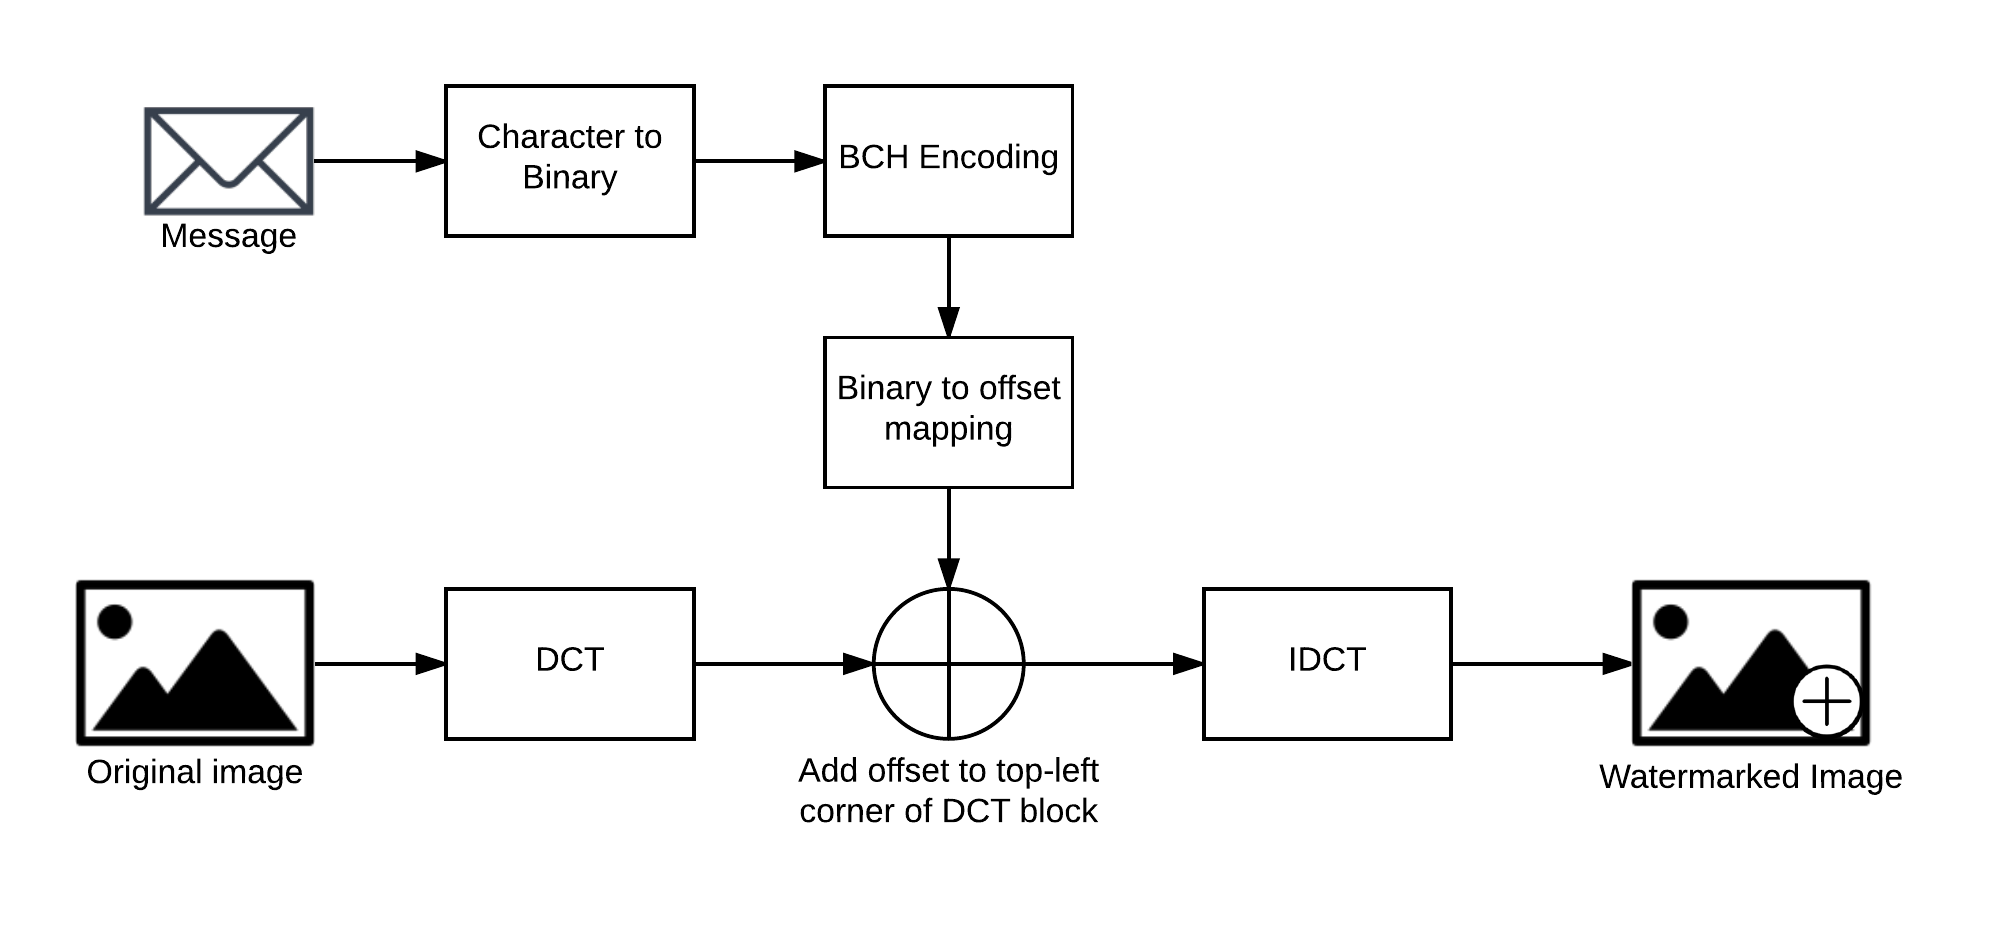
\includegraphics[width=0.75\linewidth]{graphics/encode}
  \caption{Watermark encoding process}
  \label{fig:encode}
\end{figure}

The watermark encoding function of this project is implemented through a MATLAB “m file”.
The file reads an image as input and also reads a string from the user as the watermark message.
The message must be in basic alphanumeric format and the length is limited to less than 33 characters.
This character limit is due to the requirements of the error correction methods, which will be discussed in the following sections.

The blockproc function is used to obtain the 8x8 DCT coefficients of the input image.
The watermark string is mapped letter by letter as a digit from 0 to 26, corresponding to its frequency in the english alphabet.
By employing this mapping method, we ensure that the most frequently used letters are mapped to the smallest numerical values.
The decimal values are converted to a base 6 binary format, and are then converted to a single long binary string.

In order to facilitate error correction, BCH coding was employed.
BCH coding takes a binary sequence and appends a binary correction code sequence to it.
This long binary string can be fed back into the BCH function, in the decoding stage, to produce an error-corrected binary sequence for our use in mapping back to the correct watermark message.

The binary sequence with the BCH correction code is then inserted into the top left corner of each of the DCT blocks of the image, bit by bit, as an offset.
By targeting those corners, the impact of the offsets on the quality of the overall image is minimized.
Once the watermark sequence is embedded, the image is inverse DCT and outputted to the user, ready for decoding.

\subsection{Decoding}
\begin{figure}[tbph]
  \centering
  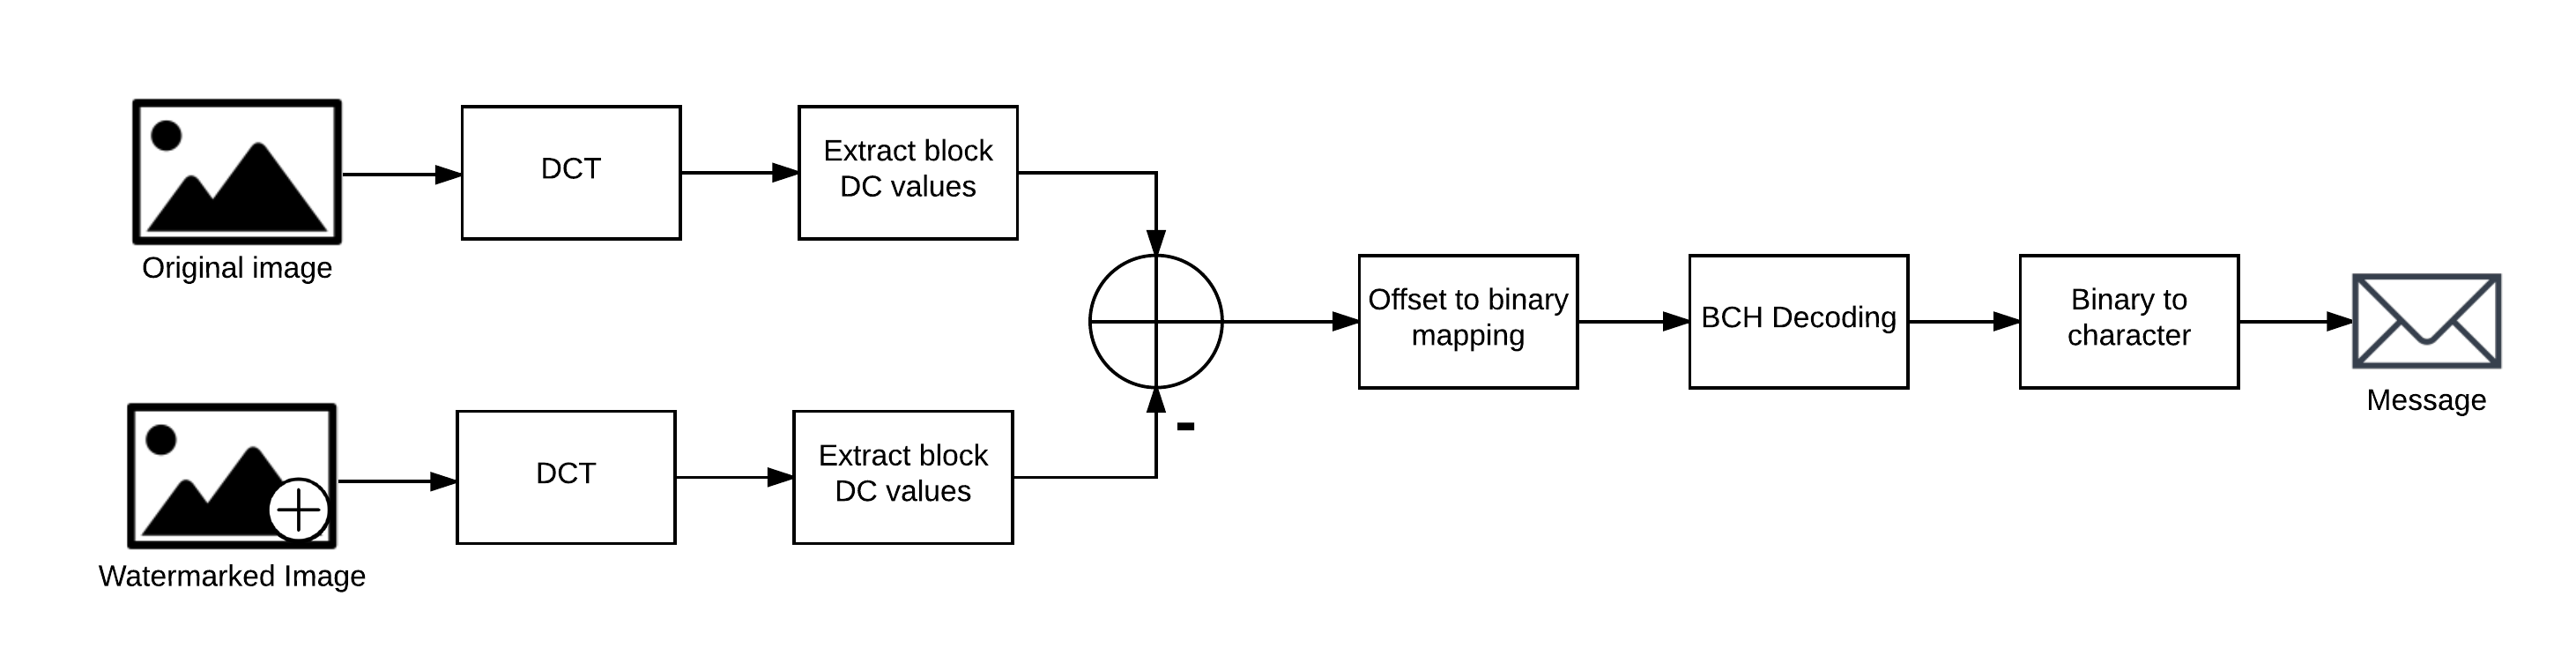
\includegraphics[width=0.95\linewidth]{graphics/decode}
  \caption{Watermark decoding process}
  \label{fig:decode}
\end{figure}

Similar to encoding, the decoding function of this project was also implemented through a MATLAB “m file”.
The file reads the watermarked image as an input, as well as the original, unwatermarked image.
The DCT coefficients of both images are acquired and the top left corner values of each block is compared to the corresponding value from the other image.
The difference is the offsets string.

This offsets string is then forced to a binary format, truncated to the correct length, and sent to through MATLAB’s BCH decoding function, where the correction code is employed in extracting the binary version of the original watermark message.
This binary code is run through an inverse mapping process and the final alphanumeric message is presented to the user as the extracted watermark.

\section{Examples}\label{sec:examples}
\stub{[Before and after images of watermark embedding}
\stub{phrases embedded vs extracted} 
\stub{PSNR comparison to embedding seq in image grayscale values}

\section{Discussion}\label{sec:discussion}
\maybe{Troubles with errors and BCH? Feel like this is covered in Implementation...}

We mention in Section~\ref{sec:intro} that the watermark cannot be removed from the image.
This does not mean that the watermark cannot be destroyed.
Since the extraction method relies on block-processing the images, any change to the block construction will drastically alter the resulting DCT.
The watermark can be destroyed trivially by removing a single row of pixels!
The security of this method relies on its ability to remain undetected.

If two parties wanted to communicate via exchange of watermarked images they would both need to have a copy of an original image to perform the message extraction.
In order to avoid creating a suspicious communication pattern where they exchange and re-exchange the same image regularly the two parties should attempt to re-use one image for multiple exchanges.
Posting ``reaction images'' and image memes on social media or other platforms would provide an excellent cover for sharing watermarked images since heavy image re-use is encouraged by the culture.

\subsection{Further work}
The motivated, row-dropping attacker problem notwithstanding, the need for an original image for decoding is a significant drawback for this method.
%Embedding the watermark so that it can be extracted without knowledge of the source image is Blind Source Separation, and is an open research problem in signal and image processing.\improvement{why is this so hard? Does this apply to our case?}
Suppose instead we used the BCH encoded message to set the DC values of the blocks to specific values that could be extracted via modular division.
The mappings would be
\begin{align*}
x^{\prime}_i = \begin{cases}
x_i + a_i \mid x_i + a_i \bmod 4 \cong 0, & m_i = 0 \\
x_i + a_i \mid x_i + a_i \bmod 4 \cong 2, & m_i = 1
\end{cases}
&&
m_i = \begin{cases}
0, & x^{\prime}_i \bmod 4 \in \{0, 1\} \\
1, & x^{\prime}_i \bmod 4 \in \{2, 3\}
\end{cases}
\end{align*}
Observe that the recovery mapping is independent of the original image $x$.
The modulus 4 is chosen avoid the casting errors described in Section~\ref{sec:enc} that would likely occur if a $0/1~\mapsto~\text{even}/\text{odd}$ mapping were used.

\section{Conclusion}\label{sec:conc}
This project succeeded in accomplishing its goal of demonstrating a procedure for watermarking digital files with almost no degradation of source image quality.
By creating a proof of concept which embedded a phrase into digital a image with minimal degradation to visual quality, and later extracted that same digital phrase with the help of BCH coding, this project demonstrated the potential and feasibility of this digital style of watermarking, in the real world.

The most obvious real world application of this technology is watermarking digital documents.
Another potential use for this methodology is in establishing a digital chain of ownership for sensitive internal documents.
Establishments will be able to keep an embedded digital record of the users who handled sensitive files. 
A record which they can trace back to the source of a leak or insurgence. Additionally, this form of embedding information in media can be used for covert communications between parties.


%%%%%%%%%%%%%%%%%%%%%%%
% 	  Referrences
%%%%%%%%%%%%%%%%%%%%%%%
\newpage
\printbibliography[heading=bibintoc,title={References}]

%%%%%%%%%%%%%%%%%%%%%%%
% 	  Back Matter
%%%%%%%%%%%%%%%%%%%%%%%
%\StartAppendices{}

\end{document}
